% ----------------------------------------------------------
% Metodologia
% ----------------------------------------------------------
\chapter{Metodologia}
\label{chap:metodologia}

O trabalho de tese em questão trata do desenvolvimento e teste
de um sistema de \textit{software}. Desse modo, a metodologia utilizada no desenvolvimento
deste sistema e, portanto, na solução do problema proposto,
é construída com base nos seguintes aspectos:

\begin{itemize}
\item Adequação das ferramentas utilizadas para alcançar o objetivo de um sistema de cálculos acoplados;
\item As restrições impostas pelas ferramentas escolhidas devido à sua estrutura intrínseca.
\end{itemize}

Desse modo, é desejável, do ponto de vista de clareza, descrever a metodologia utilizada no trabalho
apresentando as características das ferramentas utilizadas, suas limitações e seus possíveis impactos
no resultado final, de modo a então descrever a solução acoplada. Por sua vez, na descrição da solução
acoplada, são apresentadas as modificações implementadas nas ferramentas e as formas de utilização
de dois programas de computador independentes de forma conjunta.


\section{Visão Geral}

O sistema de \textit{software} desenvolvido tem algumas peculiaridades relativas à sua
implementação. Isso se deve às particularidades do problema que se pretende resolver e ao
fato não-usual de envolver duas peças de \textit{software} independentes para resolver
um problema complexo, já apresentado como um problema multi-física.

A Figura \ref{metodoetapas} apresenta uma representação gráfica do funcionamento do sistema
acoplado desenvolvido.

\begin{figure}[htb]
  \caption{Metodologia: o sistema acoplado.}
  \centering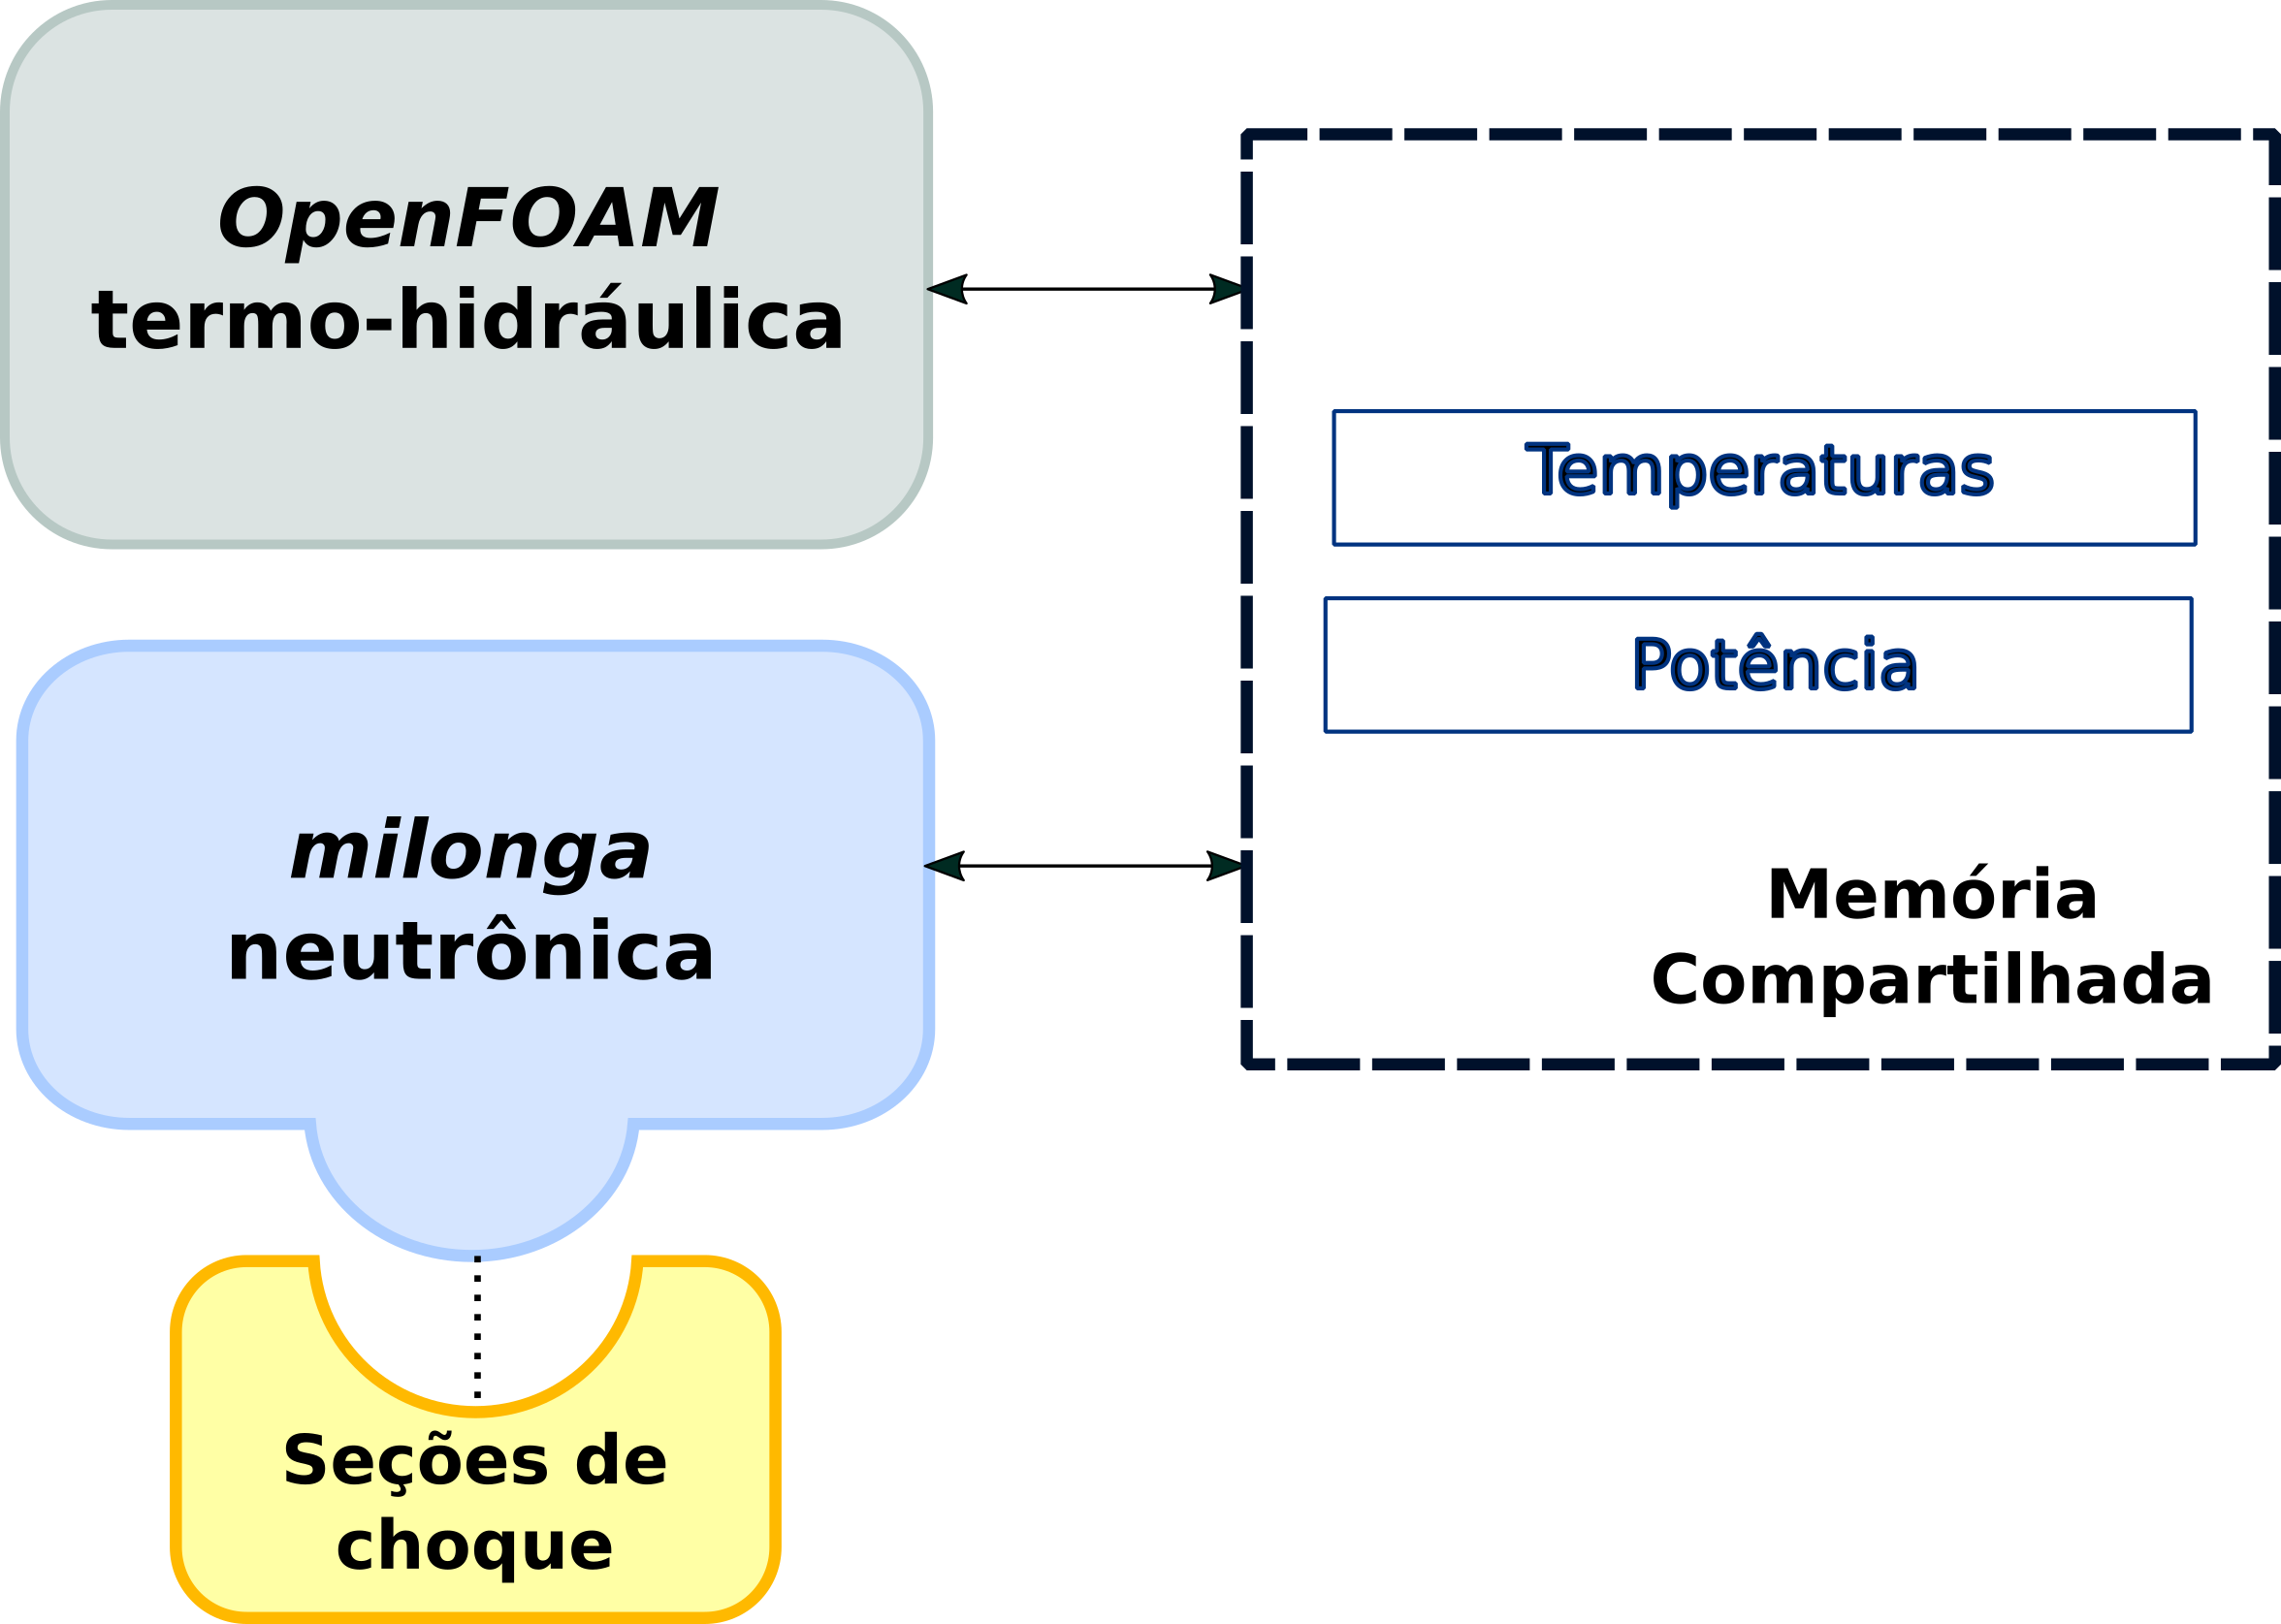
\includegraphics[scale=0.6]{figuras/metodologia2.png}
  \label{metodoetapas}
%  \legend{Fonte: autor}
\end{figure}

Como apresentado no capítulo \ref{chap:rev}, acoplamento, no contexto desta dessa tese, é a execução
de cálculos termo-hidráulicos utilizando a potência obtida pelo código de neutrônica que, por sua vez,
utiliza as temperaturas dos materiais calculadas pela termo-hidráulica para re-calcular seções de choque
e outros parâmetros neutrônicos de modo a calcular o fluxo de nêutrons e potência no combustível.

As características não-usuais desse sistema são listadas abaixo:

\begin{itemize}
\item Dois \textit{softwares} independentes interligados;
\item Uso de memória compartilhada para comunicação entre dois diferentes códigos;
\item Natureza aberta das licenças de utilização de ambos os programas (item fundamental para
  o acesso, modificação e utilização do código-fonte de ambos);
  \item Uso da mesma malha por ambos os códigos.
\end{itemize}

Nas próximas seções serão apresentadas em seus detalhes cada uma destas características que
permitiram o desenvolvimento de um sistema multi-física.

\section{Conceitos}
\label{sec:conc}

O sistema acoplado, ou multi-física, apresentado nesta tese possui algumas características
particulares já citadas. Nesta seção, serão brevemente apresentados os conceitos sobre os quais
foi possível desenhar e construir um sistema multi-física inovador com tais características.

\subsection{Multi-tarefa}
\label{subsec:mt}

Multi-tarefa é a capacidade dos sistemas operacionais de executar distintas tarefas ao mesmo tempo.
Talvez possa parecer corriqueira tal observação nos dias de hoje. Entretanto, há pouco mais de vinte
anos, a maioria dos sistemas operacionais usados em computadores pessoais não ofereciam esta
possibilidade. Em alguns casos, o que se chamou de multi-tarefa preemptiva, o usuário era capaz de
carregas distintas tarefas em memória. Contudo, apenas uma era executada por vez.

Nos sistemas computacionais atuais, em especial no sistema Linux, utilizado para o desenvolvimento
do sistema multi-física desta tese, é possível executar diversas tarefas ao mesmo tempo. Não só isso,
como há um sistema padrão de execução que permite a comunicação entre programas distintos. Diferente
de um sistema de \textit{threads} \cite{Walli1995},
em que todos os programas lançados enxergam a mesma
porção de memória, no sistema Linux cada programa tem acesso exclusivo à memória alocada para si.
Tudo isso acontece sob gerenciamento do sistema operacional.

A metodologia utilizada neste acoplamento, prevê a execução separada dos programas de termo-hidráulica
e neutrônica. Os detalhes e os algoritmos desta comunicação serão apresentados em detalhes oportunamente.
Por agora, é suficiente saber que os programas são lançados separadamente, cada qual utilizando a memória
alocada para si separadamente, sem que outros programas possam acessá-la. Dessa forma, era necessário
desenvolver um sistema ou forma de comunicação entre os códigos de neutrônica e termo-hidráulica.

\subsection{Memória compartilhada}
\label{subsec:mc}

Memória compartilhada (ou \textit{Shared-memory}) é a memória de computadores que pode ser
acessada simultaneamente por múltiplos programas em executados em diferentes
espaços de usuários com o objetivo de oferecer comunicação entre
eles evitando cópias redundantes \cite{Robbins2003}. É, ainda, uma forma eficiente
de troca de dados entre programas ou processos. A interface POSIX
(\textit{Portable Operating System Interface}) \cite{Walli1995} é um
padrão especificado pela \textit{IEEE Computer Society} para garantir
a compatibilidade entre diferentes sistemas operacionais na implementação
das formas de utilização da memória compartilhada. Para isso, é definida
uma API (\textit{Application programming interface}) que explicita as funções
e métodos de utilização da memória compartilhada. O padrão e a API disponibilizada
garatem a compatibilidade no uso dos recursos entre diferentes programas ou \textit{threads}
\cite{Atlidakis2016}.

Com mais de um programa acessando uma mesma área de memória, é necessário garantir a atomicidade
das operações por cada programa. Por atomicidade, entenda-se que uma operação iniciada por um
programa ou \textit{thread} deve ser completamente encerrada antes que outro programa ou
\textit{thread} acesse esta memória. À possibilidade de acesso concorrente ao mesmo recurso
de memória, dá-se o nome de condição de corrida.

Há diferentes técnicas para evitar condições do corrida. Dentre elas, uma das mais simples e
largamente empregada, é o uso de semáforos, inclusive usada nesta tese.
Um programa ou \textit{thread}, antes de acessar a memória
verifica se esta está livre para ser acessada. Se sim, altera o valor do semáforo enquanto opera na
memória, voltando a alterá-lo para ``livre'' ao terminar. Caso outro programa ou \textit{thread}
necessite acessar a mesma porção de memória, encontrará o semáforo em condição negativa e aguardará
um determinado tempo (definido pelo sistema operacional ou pelo próprio usuário) até tentar novamente.
Com isso, fica garantida a não-corrupção dos dados.

Deve-se dizer que há implicações negativas no uso de semáforos para controle de acesso à memória,
como por exemplo, queda de desempenho dos sistemas, em especial quando há um número grande
de programas acessando a memória compartilhada. Entretanto, a análise da possível degradação
de desempenho causada por controle de concorrência entre programas não é escopo desta tese.

Mesmo com as considerações acima apresentadas, o uso de arquivos externos para acoplamento
\cite{Hummel2016} tem tempos de acesso ordens de grandeza acima dos tempos de acesso
através de memória compartilhada \cite{Theler2013}.

\subsection{\textit{Software} livre}
\label{subsec:sl}

Muito já se disse sobre \textit{software} livre, suas características e suas licenças, como na
seção \ref{sec:intsl}. Nesta sub-seção, o objetivo se restringe às vantagens do acesso ao
código-fonte.

Ambos os códigos usados no sistema acoplado, possuem a capacidade de serem acoplados sem alterações
em seus códigos-fonte. O \textit{milonga}, em especial, já foi desenvolvido com a possibilidade
de acoplamento em mente. Portanto, oferece mais de uma forma de comunicação de dados, como por exemplo:
arquivos texto, arquivos binários e, inclusive, de forma nativa, uso de memória compartilhada.

O \textit{OpenFOAM}, entretanto, em um cenário de código fechado, só ofereceria uma forma de
acoplamento. De acordo com sua implementação, um termo-fonte só pode ser lido a cada início de
simulação. Seria, portanto necessário fazer com que o \textit{mionga} lesse os dados de temperatura
da saída do \textit{OpenFOAM}, escrevesse uma distribuição de potências em formato de entrada
para o \textit{OpenFOAM} e que este fosse novamente executado do zero. Todo esse processo, deveria
ser controlado por um \textit{script} de execução.

Apesar de soar rudimentar, está é a forma de acoplamento mais comumente empregada.
Mesmo com severo comprometimento de desempenho se comparada ao compartilhamento de
memória, técnica usada nesta tese, muitas vezes essa é a única forma de acoplamento
quando o código-fonte não está disponível \cite{Ivanov2007}.

\subsection{Discretização do domínio}
\label{subsec:dd}

A formulação utilizada para a solução da equações diferenciais que modelam o problema multi-física desta
tese é a de volumes finitos. Uma característica básica desta técnica é a utilização de pequenos volumes
de modo que as equações diferencias possam ser resolvidas como equações algébricas. A forma de obtenção
destes pequenos volumes a partir de um domínio contínuo é o que se chama \textbf{discretização de domínio}. 

A discretização do domínio significa, na prática, gerar uma malha que represente o domínio contínuo original
mantendo a conexão entre os pequenos volumes gerados. Se o domínio for tridimensional, será, geralmente,
discretizado por uma malha volumétrica. Um dos diferenciais do acoplamento apresentado está exatamente na
utilização da mesma malha para os cálculos neutrônicos, realizados pelo \textit{milonga} e termo-hidráulicos,
realizados pelo \textit{solver OpenFOAM}. Com ambos os programas utilizando a mesma malha, a relação é de um
pra um. Uma célula na neutrônica é representada exatamente pela mesma célula na termo-hidráulica.

Como mencionado anteriormente, a utilização da mesma malha para neutrônica e
termo-hidráulica é uma característica
particular do acoplamento proposto. São raros os acoplamentos com essa característica
encontrados na literatura \cite{Jareteg2014} e suas vantagens são, principalmente:

\begin{itemize}
\item Solução multi-física no mesmo nível de detalhes\footnote{Neste trabalho, se considera ``nível de detalhes'' o
  mesmo grau de discretização para ambos os problemas. O conceito pode ser estendido se for
  considerado o erro relativo dos cálculos em cada problema. Não é este o caso.};
\item Evita-se o mapeamento entre malhas que, no caso de malhas não-estruturadas, além de ser um problema de
  geometria computacional não-trivial , eventuais soluções podem acrescentar
  erros entre células \cite{Kraevoy2004}.
\end{itemize}

\subsection{Limitações}
\label{subsec:lim}

O sistema multi-física construído tem limitações, principalmente devido à limitação intrínseca de um ou de ambos
os programas usados no acoplamento. As restrições, como foram assim chamadas no início do capítulo
\ref{chap:metodologia}, são apresentadas
em forma de lista:

\begin{itemize}
\item \textbf{Sistema Operacional}: Ambos \textit{OpenFOAM} e \textit{milonga}, apesar de livremente disponíveis e,
  portanto, passíveis de utilização em diferentes sistemas operacionais são fornecidos especificamente
  para sistemas Linux. Alguns esforços recentes mostram eventuais aplicações do primeiro em sistemas
  Windows. Já para o \textit{milonga}, não há qualquer previsão de uso em outros sistemas operacionais;
\item \textbf{Execução em Paralelo}: O \textit{OpenFOAM} oferece de forma nativa a possibilidade de execução em
  paralelo. O \textit{solver} \texttt{thesisCoupledFoam} foi, inclusive, implementado de modo a funcionar em paralelo.
  Entretanto, dada a limitação do \textit{milonga}, até sua versão 0.4.65, em executar em paralelo, o sistema
  de comunicação do acoplamento está limitado a execução sequencial.
\item \textbf{Seções de choque}: a geração de seções de choque deve ser feita por algum código externo. Os
  principais códigos empregados para geração de seções de choque são fechados ou, como no
  caso do \textit{Serpent} aberto mas restrito. Entretanto, neste campo também há uma recente
  atividade no que diz respeito a \textit{software} livre. O conjunto de ferramentas \textit{PyNE},
  oferecido sob licença BSD (aberto e gratuito), tem como uma de suas propostas, a geração de seções
  de choque para aplicações de ciências nucleares e engenharia nuclear \cite{Slaybaugh20014}.:
\item \textbf{Memória}: O \textit{milonga} oferece, além da formulação de solução pela equação de difusão,
  algumas variações do método de ordenadas discretas. Entretanto, o consumo de memória e tempo de execução
  nestas formulações foi proibitivo no \textit{hardware} disponível no momento de desenvolvimento desta tese.
\end{itemize}

Apresentadas as limitações, cabe ressaltar que tais limitações, apesar de implicarem no uso,
execução e até na qualidade dos resultados dos cálculos, não são definitivas.
A quase totalidade das limitações e restrições apresentadas na lista
acima podem ser resolvidas com moderado investimento de tempo. Especificamente, tempo empregado em implementação
de novas funcionalidades como, por exemplo, a execução em paralelo do código de neutrônica ou a compilação
das ferramentas para outro sistema operacional.

Isto posto, é possível perceber que no mundo do \textit{software} limitações podem ser temporárias, de modo que um
conceito bem estabelecido pode passar antes do que se imagina, a uma ferramenta de utilização ampla.

\section{Ferramentas}
\label{sec:ferr}

Na seção anterior, foram brevemente descritos os conceitos sobre os quais foi construído
o sistema acoplado desenvolvido nesta tese. Este
sistema utiliza dois diferentes programas de computador. Cada um deles
realiza um conjunto de cálculos separadamente e compartilham os dados necessários aos cálculos do outro.

Apesar de desenvolvidos separadamente e com objetivos diferentes, algumas características comuns - além
do fato de serem ambos \textit{software} livre - permitiram seu uso acoplado. Ambos possuem a capacidade de lidar
com um mesmo formato aberto de arquivos de descrição de malhas, por exemplo.

%São dedicadas subseções a cada característica deste acoplamento definida anteriormente como não-usual.

As próximas sub-seções exploram as características destes programas que permitiram desenvolver
a metodologia neste acoplamento. São também apresentados os principais desenvolvimentos técnicos
relacionados a metodologia desenvolvida.

\subsection{Geração de malhas: \textbf{Gmsh}}
\label{subsection:gmsh}

O software \textbf{Gmsh} \cite{Geuzane2009} é um sistema gerador de malhas tridimensionais
para elementos finitos com ferramentas de pré e pós processamento. Foi desenvolvido com o objetivo
de oferecer uma ferramenta de geração de malhas rápida, leve e amigável para o usuário oferecendo,
ao mesmo tempo, capacidade de entrada de dados paramétrica e visualização. O Gmsh permite
a criação de geometrias e malhas a partir de uma interface gráfica interativa, apresentada
na Figura \ref{fig:gui-gmsh} com a malha gerada do modelo utilizado nesta tese. Outra opção
para criação de geometrias, esta mais robusta que a interface gráfica, já que permite
automatização através do uso de variáveis e estruturas simples de programação, é a leitura
de arquivos textos em formato ASCII usando sua própria linguagem interna de \textit{script}.

Assim como as outras ferramentas utilizadas no desenvolvimento do sistema acoplado desta tese,
o Gmsh é distribuído nos termos da licença GPL \cite{gplv3}. Isso equivale a dizer que
qualquer pessoa é livre para utilizar, modificar e distribuir o Gmsh, desde que não o utilize
em sistemas fechados e/ou comerciais.

% Colocar um screenshot to gmsh?
\begin{figure}[htb]
  \caption{Interface gráfica do Gmsh. }
  \centering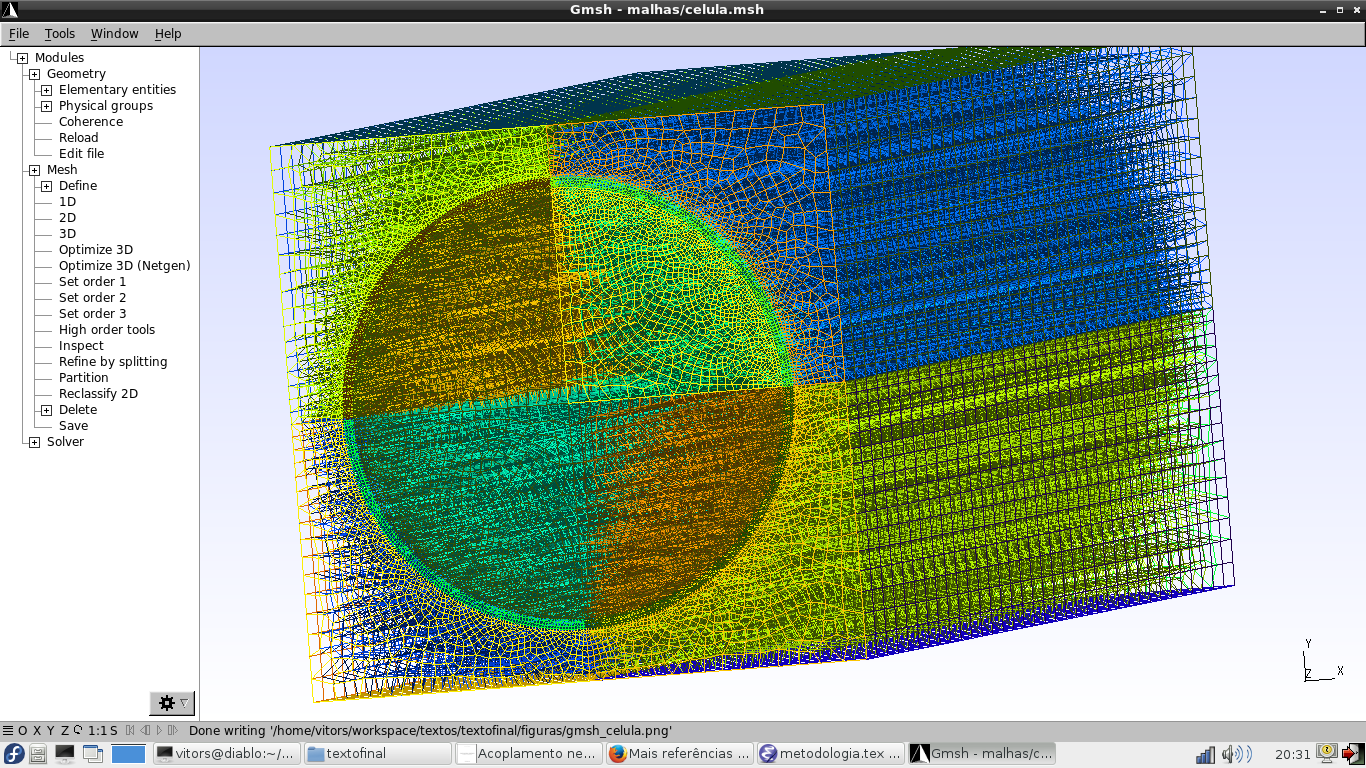
\includegraphics[scale=0.45]{figuras/gmsh_celula.png}
  \label{fig:gui-gmsh}
%  \legend{Fonte: autor}
\end{figure}


\subsection{Termo-hidráulica: \textbf{OpenFOAM}}
\label{subsection:openfoam}

O \textit{OpenFOAM} é um pacote para simulação numérica de Mecânica
do contínuo desenvolvido com base em orientação a objetos em linguagem $C++$ .
Do ponto de vista de Engenharia de Software, sua modularidade e flexibilidade são vantagens
em relação a outros códigos monolíticos  \cite{Jasak2007}. Sua implementação em componentes para manipulação de malhas, suporte
à solução de sistemas lineares, operadores de discretização e modelos físicos em forma de bibliotecas o tornam
um sistema CFD completo, aberto e gratuito. É utilizado em uma grande variedade
de aplicações, desde a solução de escoamentos complexos envolvendo reações químicas, turbulência e
transferência de calor até acústica, mecânica dos sólidos e eletromagnetismo. 

\textit{OpenFOAM} implementa um manipulador de malhas poliédrico, no qual células são descritas a partir
de um conjunto de faces fechando um volume. As faces, por sua vez, são formadas por uma lista de pontos
em suas coordenadas cartesianas e armazenados como vetores. Esta implementação é independente da discretização
usada \cite{Jasak2009}. Entretanto, as principais classes que herdam as funcionalidades das malhas implementam o método de
volumes finitos. Sendo assim, pode-se dizer que o \textit{OpenFOAM} é um sistema de CFD baseado em volumes
finitos.

Além dos componentes dedicados a operações sobre o domínio, o \textit{OpenFOAM} oferece um conjunto variado
de programas independentes chamados \textit{solvers}. Estes \textit{solvers} são dedicados à solução de
problemas físicos específicos. Para isto, utilizam outros elementos disponíveis no conjunto do
\textit{OpenFOAM}. O problema físico a ser resolvido nesta tese, especificamente do ponto de vista
termo-hidráulico, é o da solução de troca de calor conjugada entre sólidos e
fluidos distintos. Um dos \textit{solvers} que o \textit{OpenFOAM} possui com esse propósito é o
\texttt{chtMultiRegionSimpleFoam} \cite{OpenFOAM2015}.

Este \textit{solver} funciona para problemas em estado estacionário e para
fluidos compressíveis. A modularidade do \textit{OpenFOAM}
fica clara na forma como o \textit{solver} interage com os outros módulos: para regiões sólidas,
são utilizados modulos de propriedades termo-físicas específicos para sólidos. Por sua vez, para
fluidos são oferecidos outros módulos com implementações relativas a propriedades de fluidos.
Outro exemplo é a utilização de turbulência: caso o usuário estabeleça que seu escoamento é laminar,
o módulo para escoamentos laminares é utilizado. Caso o escoamento seja turbulento, o usuário pode
escolher entre implementações de diferentes modelos de turbulência.

O \textit{solver} utilizado permite escolher entre energia interna e entalpia para a solução
da equação da energia, de acordo com o módulo termodinâmico escolhido. Na implementação do
problema acoplado, foi usada entalpia. O modelo de turbulência utilizado foi o $\kappa-\epsilon$
\cite{Launder1974}.

%Mais detalhes as características do escoamento simulado e do modelo de turbulência serão
%discutidos no capítulo \ref{chap:aplicacao} e sub-seção \ref{subsec:turb}, respectivamente.

O \textit{OpenFOAM} é capaz de importar malhas no formato aberto \textbf{gmsh} \cite{Geuzane2009}. Este
formato é o mesmo utilizado pelo \textit{milonga} para leitura de malhas não-estruturadas.



% -----------------------------------------------------------------------------------------------------

\subsection{Neutrônica: \textbf{milonga}}
\label{subs:milonga}

O \textit{milonga} é um \textit{software} aberto e livre para cálculo de física de reatores
liberado sob licença to tipo GNU \cite{gplv3}. Ele é construído utilizando-se de bibliotecas
conhecidas como a \textit{GNU Scientific Library} \cite{Galassi2009}, a biblioteca
PETSc \cite{Balay2016} e na biblioteca para solução de problemas da autovalores e autovetores
SLEPc \cite{Hernandez2005}. A re-utilização de bibliotecas consagradas traz robustez para
o \textit{milonga}, ao mesmo tempo seguindo os princípios do desenvolvimento de \textit{software} livre.

O \textit{milonga} resolve a equação de transporte de nêutrons multi-grupos em estado estacionário,
utilizando a aproximação por difusão ou o método de ordenadas discretas. Oferece dois esquemas
de discretização, elementos e volumes finitos. A capacidade de utilizar volumes finitos em malhas
não-estruturadas permite sua utilização de forma acoplada com o \textit{ÒpenFOAM}. O formato
de leitura de malhas não-estruturados utilizado pelo \textit{milonga} é o \textbf{gmsh}, formato
este que o \textit{OpenFOAM} é capaz de importar, como mencionado anteriormente.

Dentre as distintas formas de resolver a equação de transporte oferecidas pelo \textit{milonga},
optou-se por utilizar a aproximação por difusão. Apesar de resultados inacurados e das limitações
na sua utilização em algumas circunstâncias \cite{Trahan2014}, a aproximação por difusão
foi o modelo escolhido devido à sua execução mais rápida e menor consumo de memória.
A aproximação por difusão é apresentada na equação \ref{eq:difusao} já na sua forma discretizada
para $G$ grupos:

\begin{equation}
  \label{eq:difusao}
  \begin{split}
  & 0 = \nabla . \big[D_g({\bar{x}}) \nabla \phi_g(\bar{x})\big] 
- \Sigma_{tg}(\bar{x}).\phi(\bar{x}) \\
& + \sum_{g'=1}^{G} \Sigma_{sg'\rightarrow g}(\bar{x}) . \phi_{g'}(\bar{x})
+ \chi(g)  \sum_{g'=1}^{G} \frac{\nu \Sigma_{fg'}(\bar{x})}{k_{eff}} . \phi_{g'}(\bar{x}) \\
  \end{split}
  \end{equation}

(Inserir a tabela de grandezas)

% -----------------------------------------------------
% Adicionado depois da conversa com a Cláubia dia 24/11
% -----------------------------------------------------
Nessa formulação, espera-se que as seções de choque macroscópicas e os coeficientes de difusão sejam
previamente computador por códigos de \textit{lattice} para serem usados na formulação por difusão.
A dependência das seções de choque da temperatura pode ser considerada linear uma vez que
os coeficientes são mantidos constantes durantes cada passo do cálculo iterativo utilizado
pelo \textit{milonga}.

A equação \ref{eq:difusao} assume que todos os coeficientes de difusão utilizados são
contínuos no espaço. Na formulação de volumes finitos,
o fluxo escalar é definido em cada célula. Quando células vizinhas são formadas
pelo mesmo material, é possível estimar o módulo do gradiente do fluxo
utilizando o teorema do valor médio \cite{Theler2013b}.

Caso isso não seja verdade, então o operador de divergência não
está definido nos pontos de discontinuidade. Assim, a formulação apresentada precisa tratar
dos casos de descontinuidade, que são, na prática, as superfícies de fronteiras entre
materiais. Nessas interfaces, o \textit{milonga} aplica uma condição de
conservação da corrente de neutrons:

\begin{equation}
  \label{eq:corrente}
  D_g^+(\bar{x}).\nabla \phi_g^+(\bar{x})=D_g^+(\bar{x}).\nabla \phi_g^-(\bar{x})
  \end{equation}

Na equação \ref{eq:corrente}, os sinais de mais e menos representam os lados da
interface. Como os coeficientes de difusão são diferentes, a distribuição de
fluxo $\phi_g(\bar{x})$ resultante deve ter um gradiente descontínuo na
interface de modo a conservar a corrente. Na formulação de volumes finitos,
no caso de células vizinhas compostas por materiais diferentes, espera-se que
o coeficiente de difusão $\phi_g(\bar{x})$ não seja contínuo na interface
entre as células. O que se aplica, neste caso, é outro estimador do módulo
do gradiente, de modo que o fluxo na superfície seja o mesmo visto de um volume
da interface quanto do outro. Esta estimativa leva em consideração os volumes e
a geometria das células envolvidas. Uma explicação elegante com o formalismo
matemático utilizado na implementação do método de volumes finitos no
\textit{milonga} pode ser encontrada no trabalho de Theler \cite[Seção 3.5.2]{Theler2016}.


%Com base na corrente, é implementada
%uma condição de contorno de \textit{albedo}. Sendo as correntes em cada lado
%da interface, respectivamente,

%\begin{equation}
%  \label{eq:corrente-albedo+}
%  J_g^+(\bar{x})=D_g^+(\bar{x}).\nabla \phi_g^+(\bar{x})
%\end{equation}

%\begin{equation}
%  \label{eq:corrente-albedo-}
%  J_g^-(\bar{x})=D_g^-(\bar{x}).\nabla \phi_g^-(\bar{x})
%\end{equation}

%O albedo em $(\bar{x})$ é definido pela relação

%\begin{equation}
%  \label{eq:albedo}
%\beta_g(\bar{x})=\frac{J_g^-(\bar{x})}{J_g^+(\bar{x})}
%\end{equation}

%Com base no \textit{albedo}, é implementada uma condição de contorno capaz de lidar
%com a descontinuidade entre regiões com diferentes propriedades. A implementação
%das condições de contorno, bem como detalhes das formulações de volumes e elementos
%finitos utilizados no milonga são elegantemente explicados por Theler \cite{Theler2013b}.
%Detalhes sobre a continuidade de condições de contorno e a suas formas de implementação
%na equação de difusão em estado estacionário são cuidadosamente apresentados por Hébert
%\cite{Hebert2009}.

De forma padrão, o \textit{milonga} funciona lendo um arquivo de entrada que modela o
problema a ser resolvido. Um dos casos mais simples em que se resolve o fluxo de nêutrons
num sistema crítico, com seções de choque constantes, é apresentado na figura \ref{fig:inputmilonga}.
Pode-se observar a definição da formulação, esquema de solução e número de grupos na linha 7.
Os coeficientes da equação de difusão para um material são apresentadas nas linhas 10-16.
Condições de contorno baseadas na malha estão definidas nas linhas 19-21 e, na linha 24,
está o comando utilizado para iniciar os cálculos.

Além dos comandos apresentados, o \textit{milonga} possui um vasto conjunto de comandos e primitivas
que vão desde pré-processamento da malha até primitivas de saída para visualização gráfica da
solução.

\begin{figure}[htb]
  \caption{Arquivo de entrada básico do milonga. }
  \centering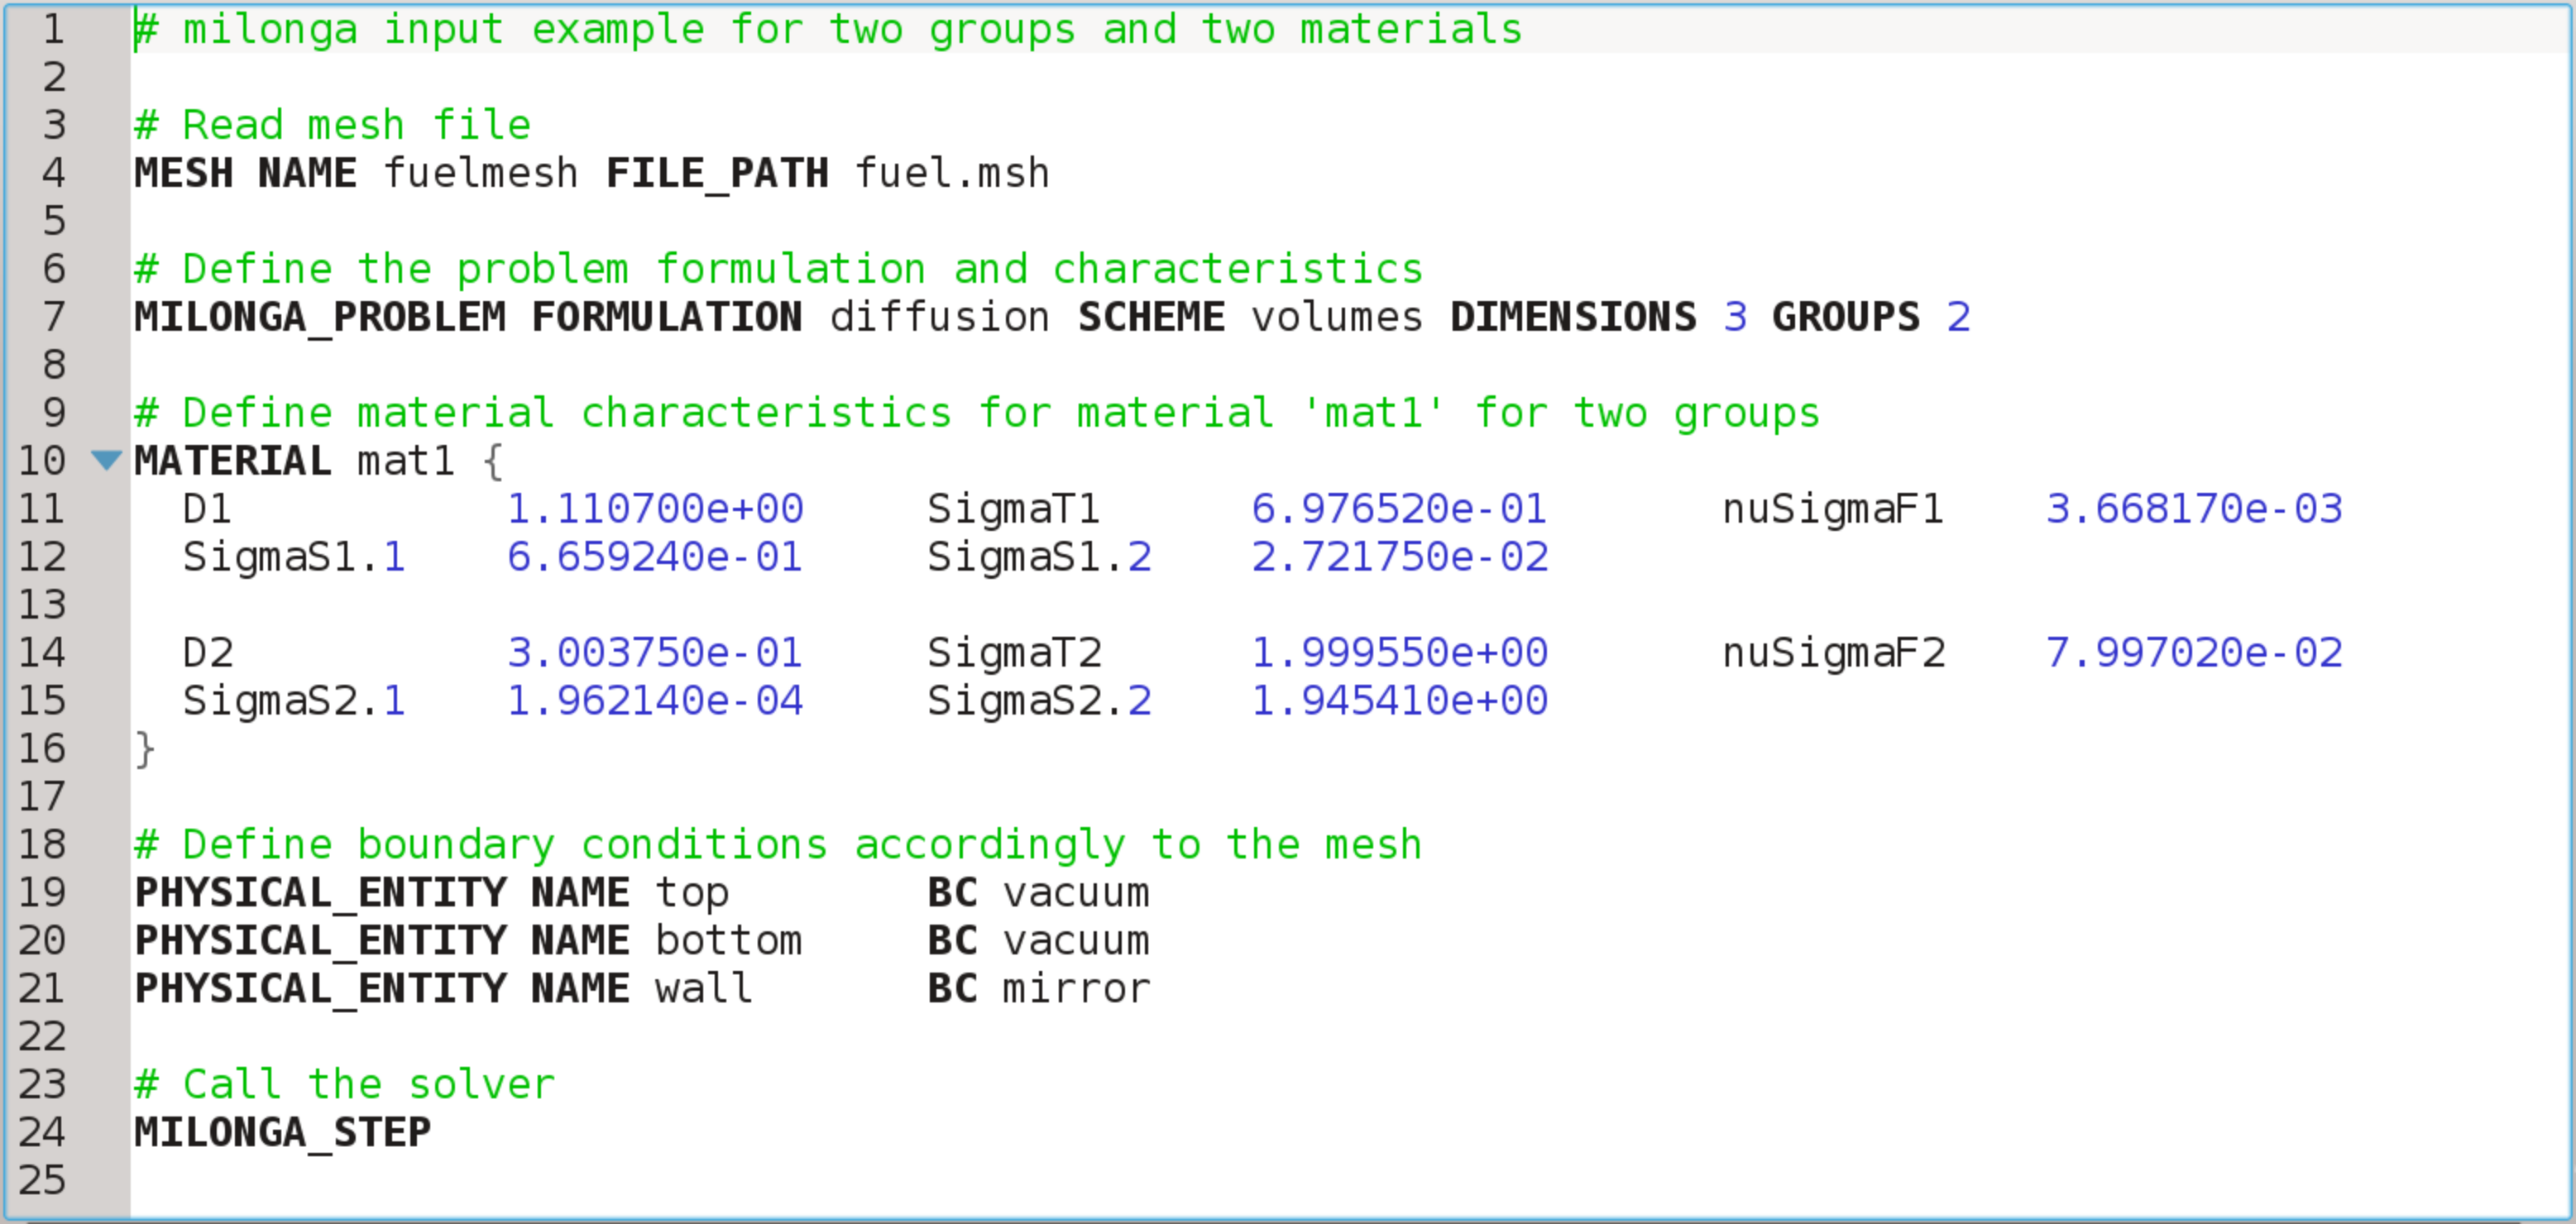
\includegraphics[scale=0.19]{figuras/milonga_example2.png}
  \label{fig:inputmilonga}
%  \legend{Fonte: autor}
\end{figure}

Uma funcionalidade fundamental do \textit{milonga} para o acoplamento neutrônico
e termo-hidráulico é a possibilidade de definir as seções de choque como expressões
algébricas de $x$, $y$ e $z$, como funções definidas geometricamente em $x$, $y$ e $z$
ou como combinação de ambos os métodos. Para o acoplamento, em especial, a definição
de funções geometricamente permite estabelecer valores para os coeficientes de
acordo com a posição da célula na malha. A aplicação é ainda mais extensa, já que
uma vez que é possível utilizar expressões pela posição na malha, é também
possível definir concetração de veneno ou fração de vazio por elemento da malha.

Além disso, o \textit{milonga} pode ser dados em tempo de execução de arquivos de
entrada, arquivos binários e, em especial no contexto desta tese, de memória compartilhada.
Esta é uma funcionalidade deste \textit{software} que o torna preparado para uso de
forma acoplada.


\section{Acoplamento}
\label{sec:acoplamento}

Sabe-se, neste ponto, que os dois programas, \textit{milonga} e \textit{OpenFOAM} funcionam
independentemente e utilizam uma parte da memória do computador de forma compartilhada.
Nesta seção, são apresentados os detalhes algoritmicos desta comunicação entre neutrônica e
termo-hidráulica.

Como funcionam separadamente, é necessário estabelecer, além dos dados a serem compartilhados
como ambos os códigos irão se comportar. A opção utilizada - e aqui cabe um comentário: há diversas
formas de definir as bases de execução dos dois programas. Neste trabalho, optou-se por utilizar,
dentre as propostas, a mais simples. Esta solução consiste em executar o \textit{milonga}, que aguarda
o a inicialização do \textit{OpenFOAM}. Os programas podem ser lançados em diferentes janelas ou
na mesma janela em \textit{background}, já que o funcionamento da memória compartilhada é independente,
inclusive, do usuário que lançou o programa.

As próximas seções apresentam o algoritmo de acoplagem para cada código separadamente.


% -------------------------------------------------------------------------------------------------------------
\subsection{Algoritmo termo-hidráulica}
\label{subsec:th}

O algoritmo de acoplamento do \textit{solver} \texttt{thesisCoupledFoam} está implementado
via código-fonte. Apesar de ser possível utilizar de referências ao código-fonte para
apresentar o algoritmo, como feito para a implementação do termo-fonte na seção \ref{subsec:detth},
esta forma é um pouco árida. Sendo assim, os algoritmos de acoplamento, para ambos os códigos,
serão descritos por meio de pseudo-código.

A Figura \ref{fig:algo_th} apresenta o algoritmo de acoplamento para o \textit{OpenFOAM}.
As expressões em azul escuro mostram as instruções relativas ao uso de memória compartilhada,
enquanto em vermelho estão as instruções relativas ao controle de acesso aos dados (semáforos).
É possível notar, em relação à Figura \ref{fig:algo_th}, três principais divisões:

\begin{figure}[htb]
  \caption{Algoritmo termo-hidráulica.}
  \centering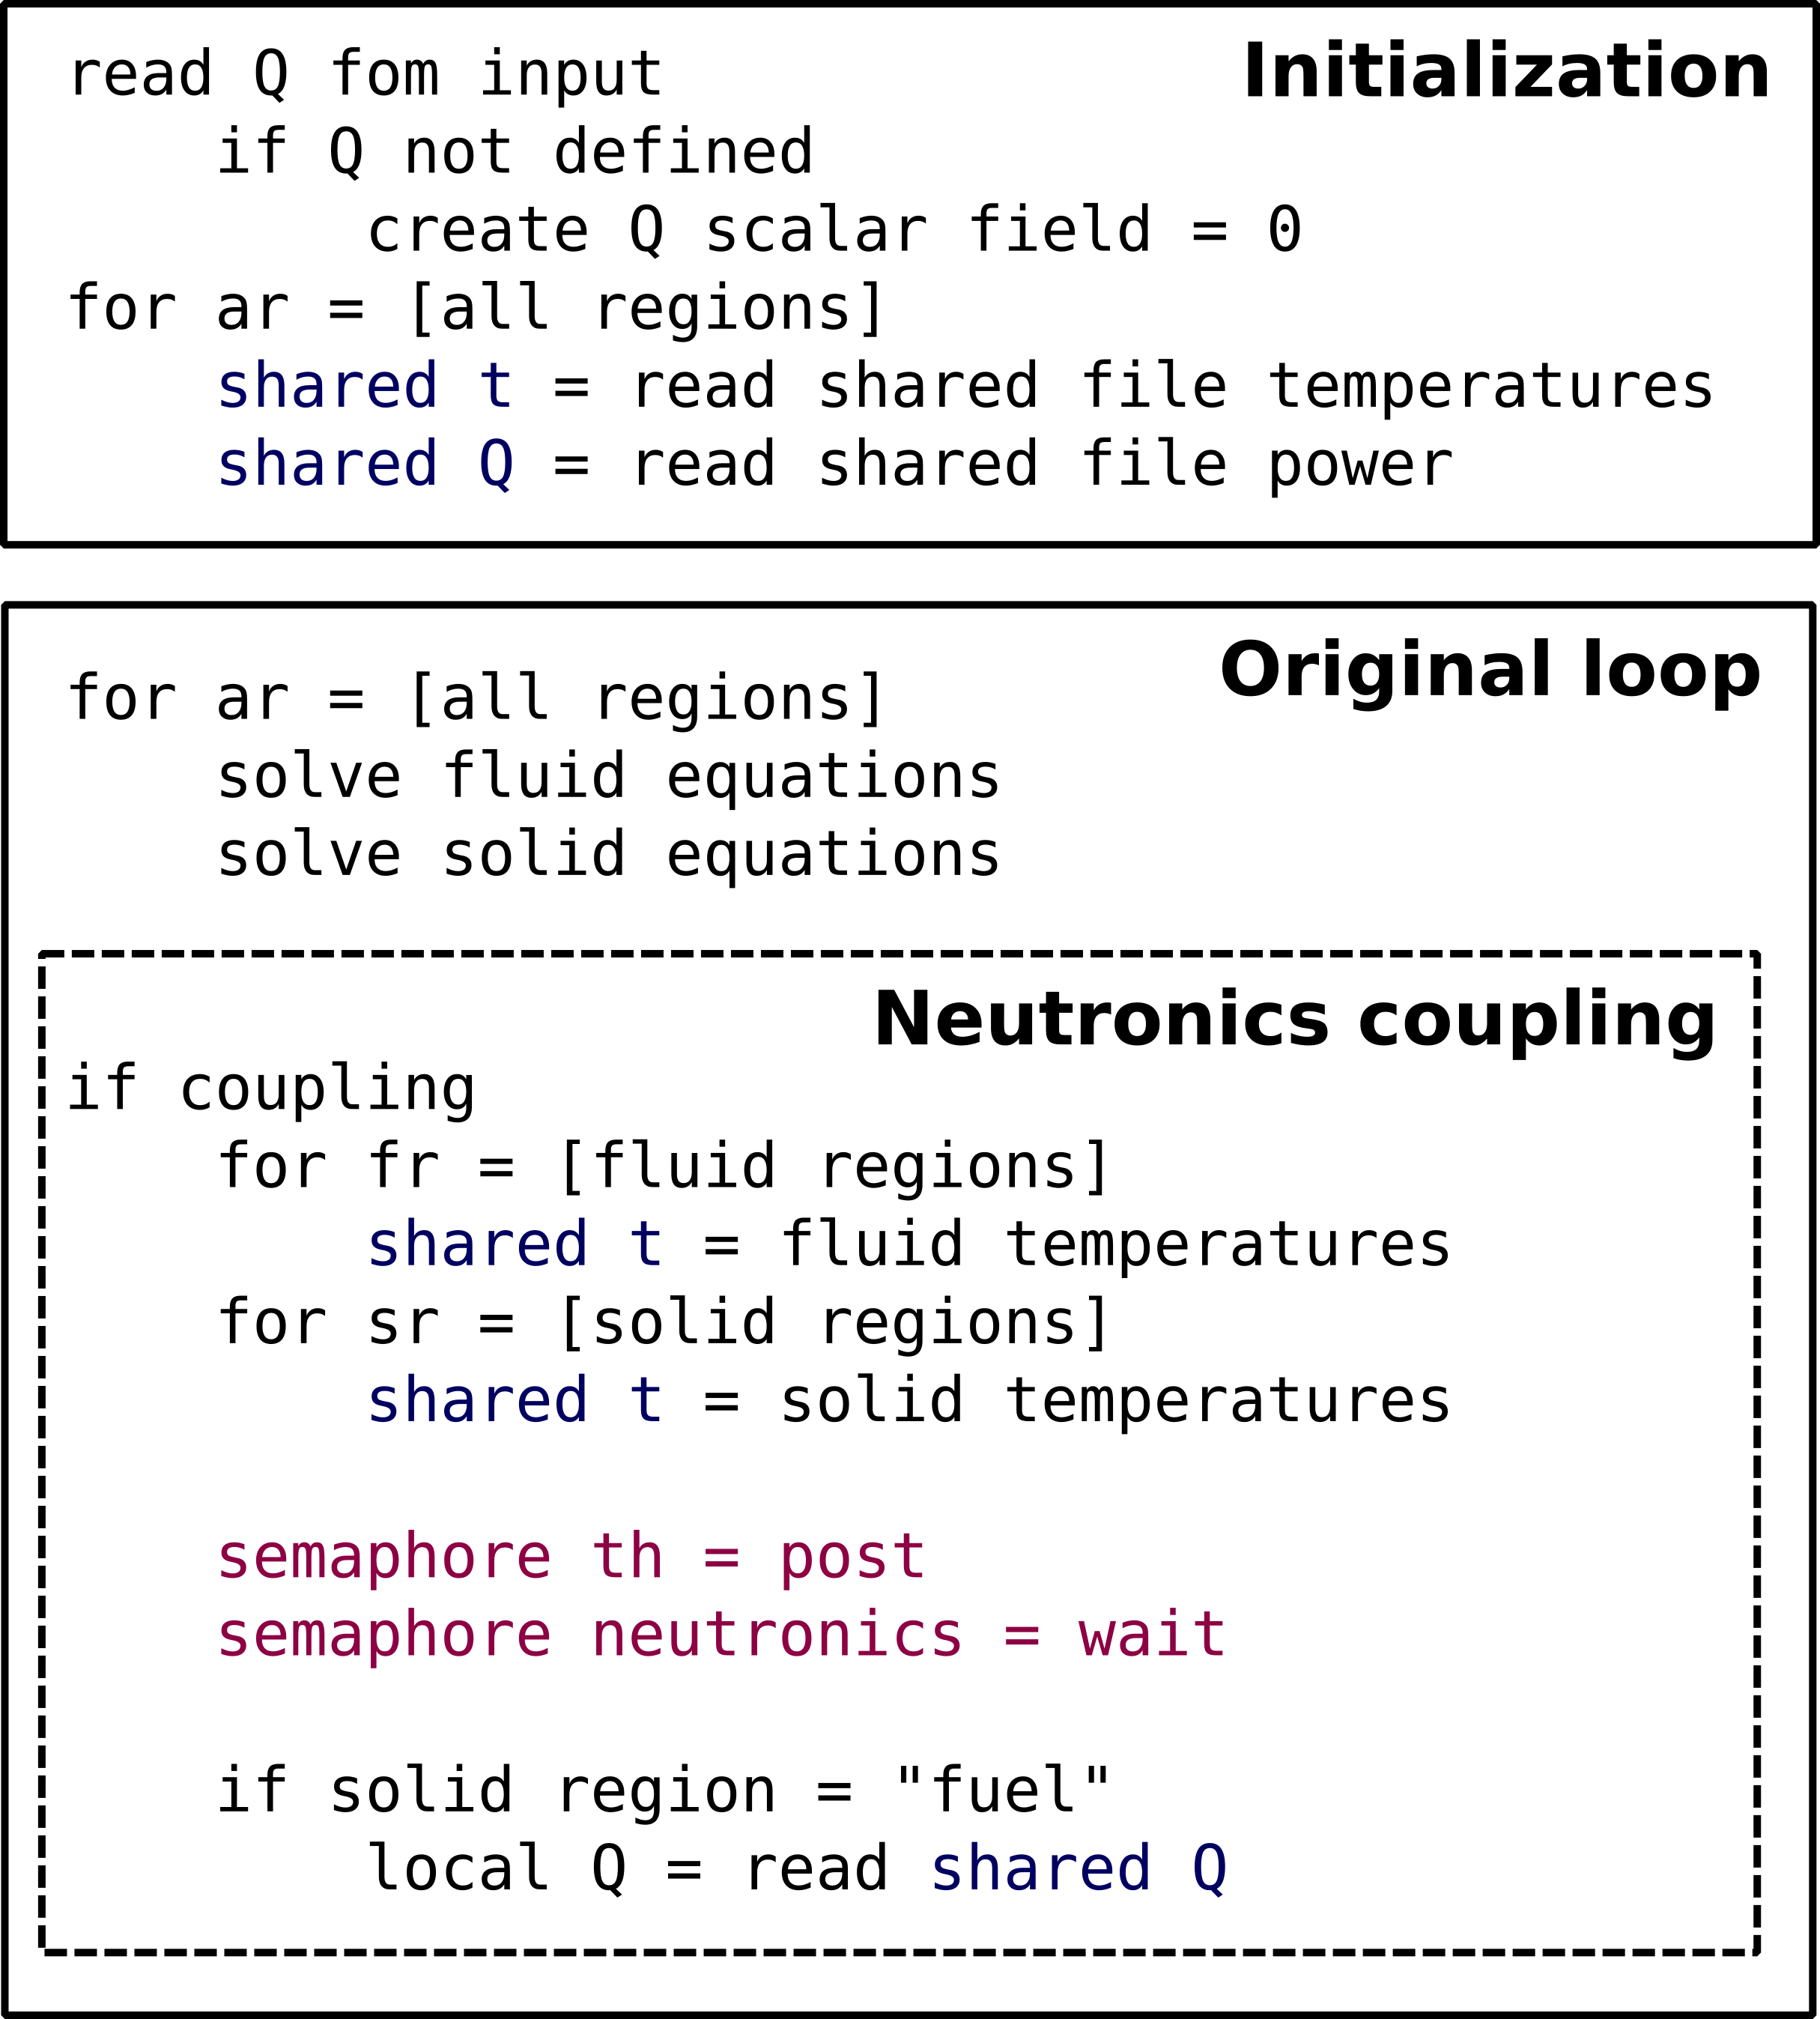
\includegraphics[scale=0.5]{figuras/algoritmo_openfoam.png}
  \label{fig:algo_th}
%  \legend{Fonte: autor}
\end{figure}

\begin{itemize}
\item \textbf{Inicialização:} Na inicialização do \textit{OpenFOAM}, é lido o valor inicial da potência para
  a simulação caso o arquivo de definição de potência esteja disponível. Caso contrário, a potência é inicializado
  com zero. Os espaços em memória compartilhada são verificados. Caso não estejam corretamente alocados, o sistema
  assume que o sistema executará de forma não-acoplada. Cabe lembrar, como dito no início da seção \ref{sec:acoplamento},
  o \textit{milonga} é iniciado antes do \textit{OpenFOAM} e, conforme será descrito no algoritmo da neutrônica, é
  ele o encarregado da alocação da memória compartilhada.

\item \textbf{Laço original:} Este é o laço do \textit{solver} original na sua execução do algoritmo SIMPLE. Este
  trecho não foi alterado em relação ao original e nesta etapa são resolvidas as respectivas equações
  para as regiões fluidas e sólidas. Ao fim
  deste laço, os valores de temperatura de cada célula de cada região estão calculados e disponíveis.

\item \textbf{Acoplamento com a neutrônica:} Caso seja o momento de troca de dados (a implementação atual
  executa uma chamada acoplada para cada 100 iterações da termo-hidráulica), para as regiões fluidas são copiados os valores
  de temperaturas para a memória compartilhada nas posições relativas às células das regiões fluidas. Em seguida, o mesmo
  é feito para as regiões sólidas. Com os valores calculados disponíveis na memória compartilhada, o \textit{OpenFOAM}
  avisa (post) no semáforo relativo à termo-hidráulica (th) que a memória compartilhada está liberada para uso. No próximo
  passo o \textit{OpenFOAM} lê o semáforo da neutrônica que, neste instante, indica que o \textit{OpenFOAM} aguarde. Quando
  receber o aviso (post) de liberação, o \textit{OpenFOAM} continua e, apenas para a região nomeada como combustível (fuel),
  lê os dados de potência disponíveis na memória compartilhada para sua estrutura de dados local, um campo escalar volumétrico
  de potências.
\end{itemize}

Ao fim da execução da etapa relativa ao acoplamento, o controle de execução volta ao laço original. A inicialização é
feita uma única vez para todos os passos de simulação.

% -------------------------------------------------------------------------------------------------------------
\subsection{Algoritmo neutrônica}

No caso da neutrônica, não há necessidade de alterações no código-fonte do \textit{milonga}. Absolutamente
todo o controle do algoritmo de acoplamento é feito no arquivo de entrada. Na versão do
\textit{milonga} utilizada (0.4.65) as opções de utilização iterativa ainda são limitadas. Estruturas
de repetição utilizando condicionais não estão disponíveis. Com isso, optou-se por definir um laço com número
de execuções fixa. A partir dessa restrição, foi desenvolvido o algoritmo de execução. A figura
\ref{fig:algo_neutronica} mostra o algoritmo e suas etapas. As expressões em azul escuro mostram as instru-
ções relativas ao uso de memória compartilhada, enquanto em vermelho estão
as instruções relativas ao controle de acesso aos dados (semáforos). Cabe ressaltar que,
como mencionado anteriormente,
o \textit{milonga} é iniciado \textbf{antes} do \textit{OpenFOAM}.

\begin{figure}[htb]
  \caption{Algoritmo neutrônica.}
  \centering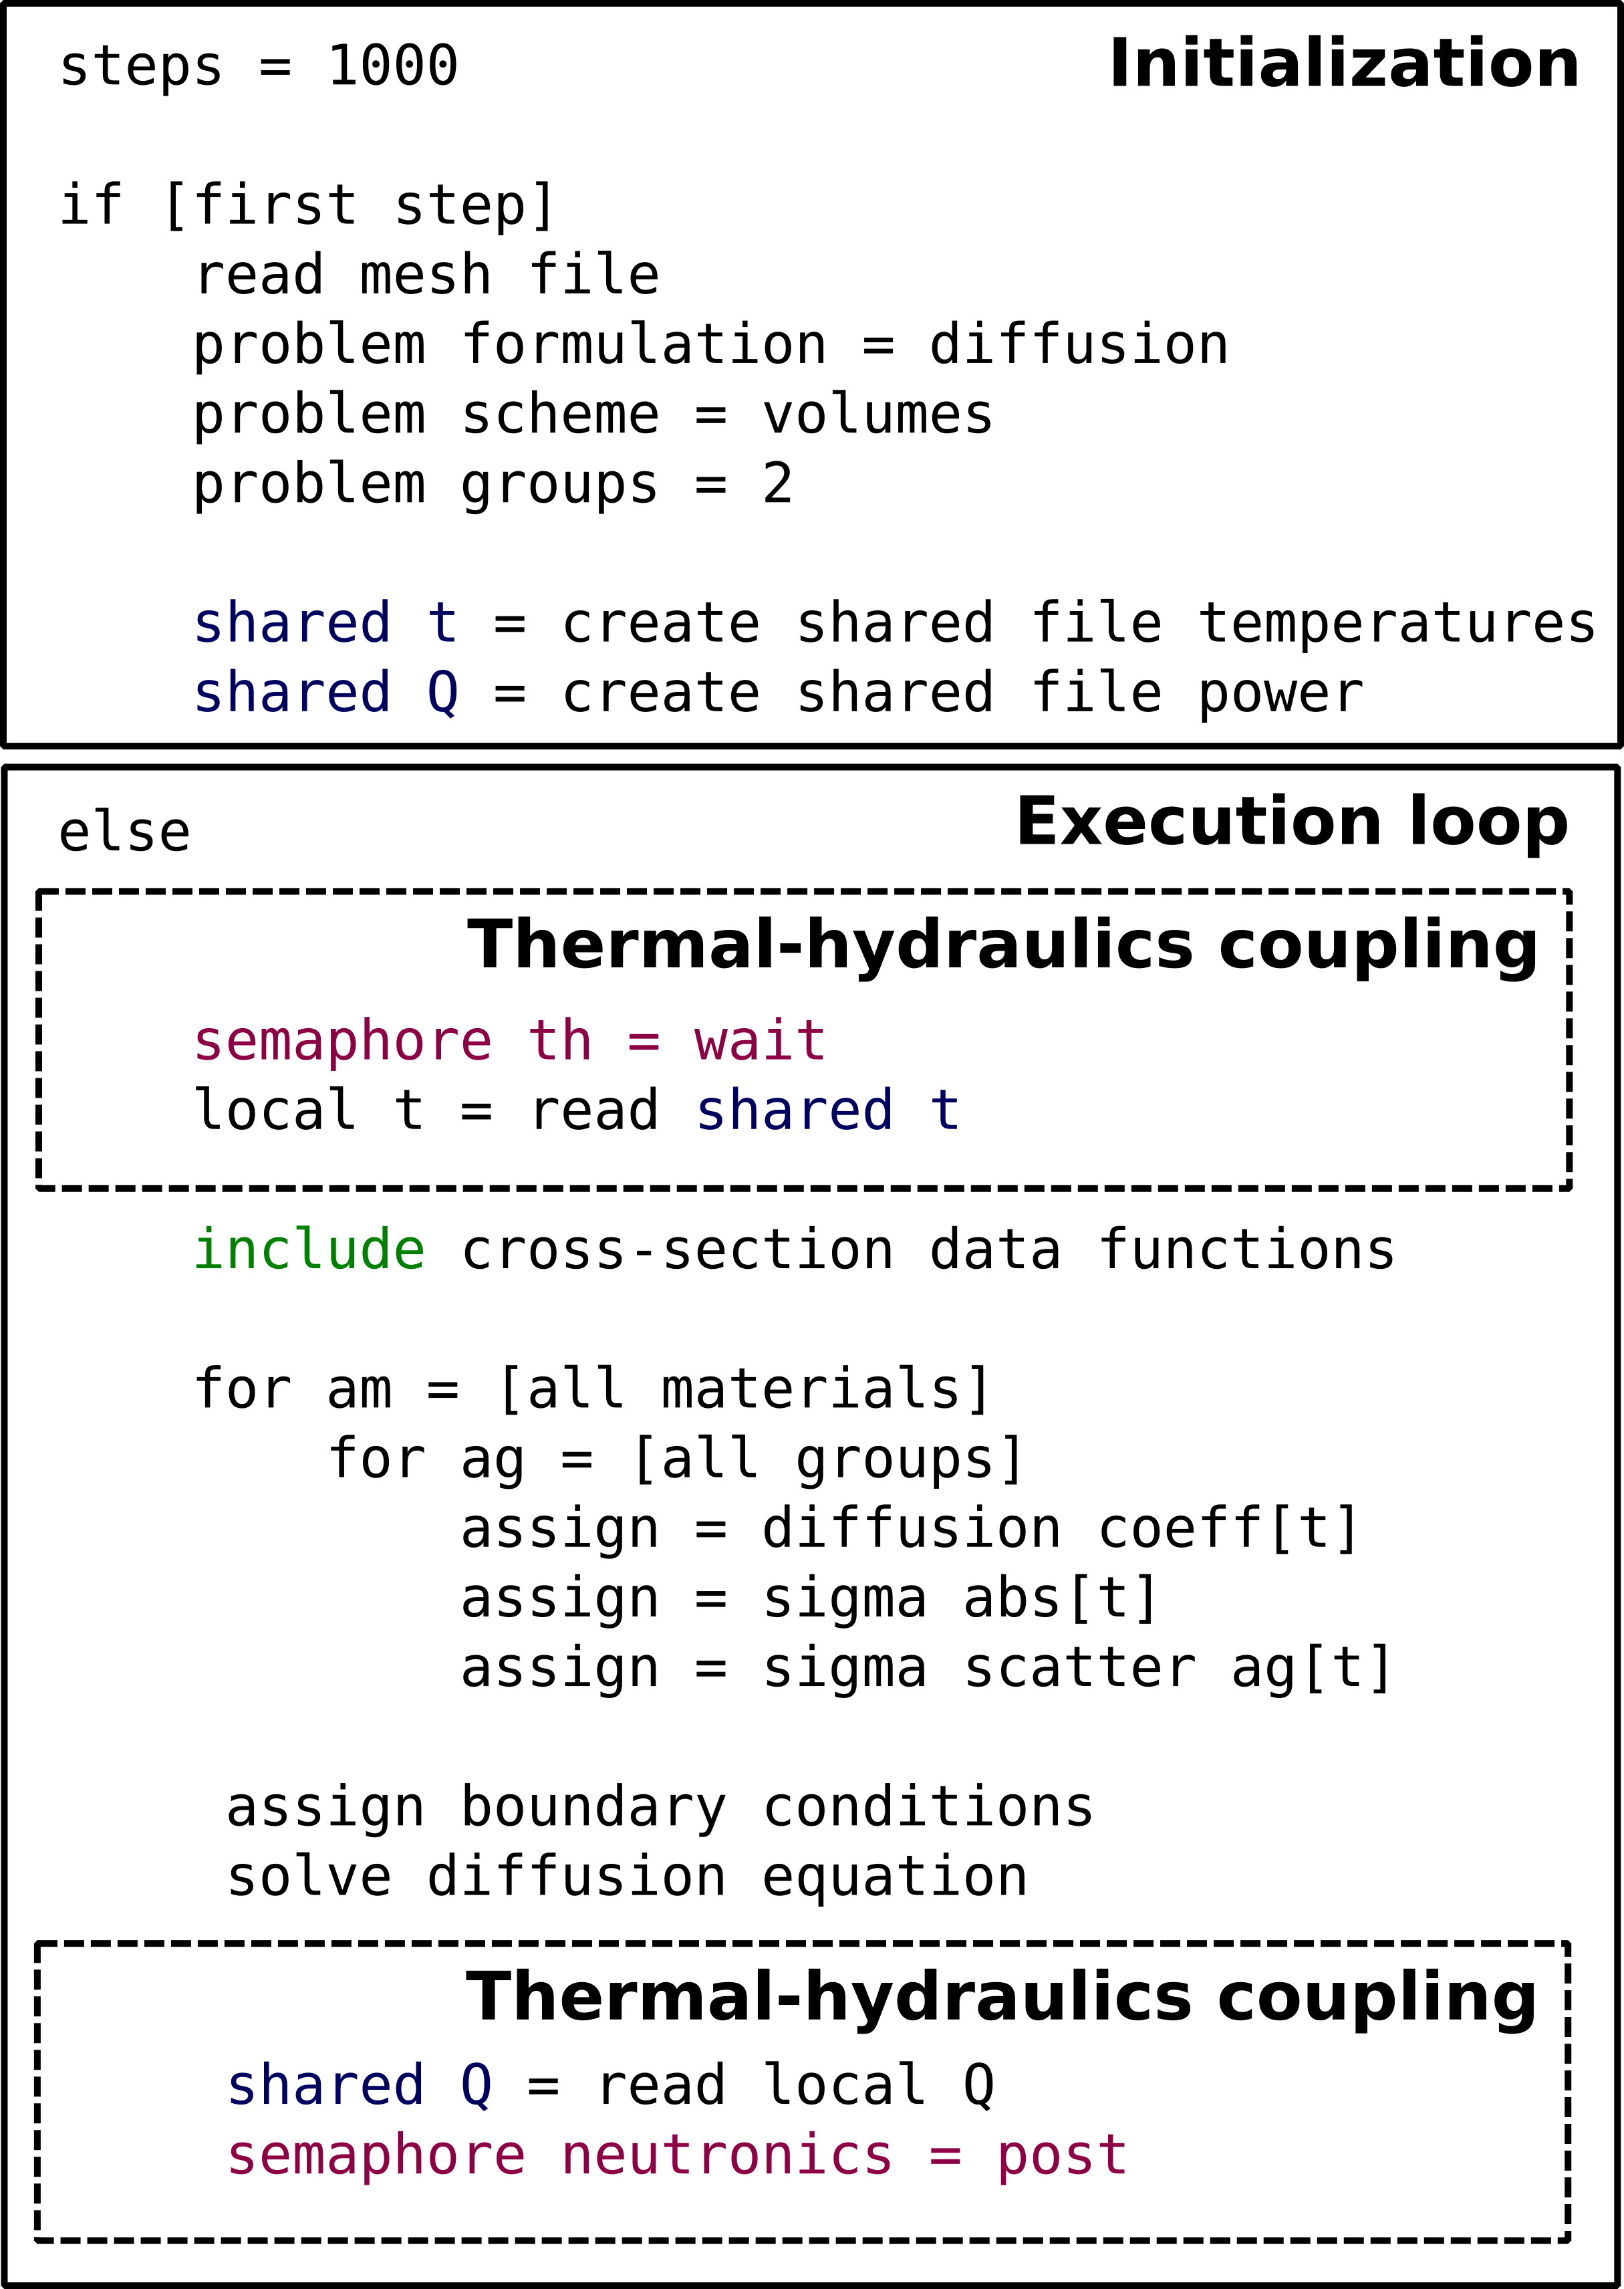
\includegraphics[scale=0.5]{figuras/algoritmos_milonga.png}
  \label{fig:algo_neutronica}
  %  \legend{Fonte: autor}
\end{figure}

\begin{itemize}
\item \textbf{Inicialização:} É definido o número de iterações a serem executadas - obrigatoriamente maior do que o número
  de vezes que o \textit{OpenFOAM} fará chamadas ao \textit{milonga}. Caso seja o primeiro passo, o \textit{milonga}
  lê a malha, estabelece a formulação matemática, o esquema de discretização e o número de grupos de energia, exatamente
  como apresentado na figura \ref{fig:inputmilonga}. A seguir, através das primitivas de utilização de memória compartilhada
  presentes no \textit{milonga}, são criadas areas em memória compartilhada para armazenar temperaturas e potência. Os tamanhos
  destas áreas são obtidos do tamanho da malha carregada anteriormente. A inicialização, como é de se esperar, é feita uma única
  vez durante toda a simulação acoplada.
\end{itemize}

As instruções referentes ao acoplamento em si, ou seja, acesso à memória compartilhada e semáforos
(caixas hachuradas na figura \ref{fig:algo_neutronica}) estão localizadas dentro do laço de execução e serão
descritas na explicação deste.

\begin{itemize}
\item \textbf{Laço de execução:}

\begin{itemize}
\item \textbf{Acoplamento termo-hidráulico:} A execução dos cálculos do neutrônicos se inicia com a leitura do semáforo da
  termo-hidráulica, o que faz com que o \textit{milonga} pare, aguardando os resultados dos cálculos termo-hidráulicos.
  Quando recebe a sinalização de que é possível prosseguir, o \textit{milonga} armazena em sua estrutura interna os dados
  de temperatura provenientes da termo-hidráulica disponíveis na memória compartilhada.
\item Cálculo neutrônico: São lidas as funções que armazenam seções de choque e todos os coeficientes previamente calculados para quatro
  diferentes temperaturas. Assim, para todos os materiais e para todos os grupos são atribuídos os coeficientes de difusão,
  seções de choque de absorção e seções de choque de espalhamento para cada célula, em função da temperatura da célula.
  Em seguida, são atribuídas as condições de contorno do problema neutrônico e iniciada a solução do problema.
\item \textbf{Acoplamento termo-hidráulico:} Antes do fim do laço, com o problema neutrônico resolvido, fluxos e potência
  calculados, os valores de potência são escritos na memória compartilhada e então o \textit{milonga} avisa (post) no
  semáforo relativo à neutrônica (neut) que a memória compartilhada está disponível para uso.

\end{itemize}
\end{itemize}

Ao fim da simulação termo-hidráulica, o \textit{milonga} permanece parado. Para finalizá-lo deve ser enviado um sinal de
cancelamento de execução via teclado. Todo o procedimento de acoplamento da neutrônica é feito por meio de um arquivo
de entrada, sem necessidade de alteração do código-fonte e compilação, sempre interpretado em tempo de execução.

% -------------------------------------------------------------------------------------------------------
\subsection{Implementação: uma olhada no código-fonte.}
\label{subsec:detth}
Na seção \ref{sec:th} foram apresentadas as bases teóricas do problema termo-hidráulico.
Nesta sub-seção, são
descritas as alterações diversas promovidas no \textit{solver} original do \textit{OpenFOAM}
que foi chamado \texttt{thesisCoupledFoam}.

A principal alteração feita no \textit{solver} originalmente implementado foi a adição de um termo-fonte.
Esta alteração permite a geração de calor no sólido, útil tanto no problema acoplado
quanto numa eventual simulação isolada em que se deseje geração de
calor\footnote{A partir da versão 2.2, o \textit{OpenFOAM} introduziu em alguns dos seus
\textit{solvers}, incluindo o \texttt{chtMultiRegionSimpleFoam}, a possibilidade de definição
de termo-fonte via \texttt{fvOptions}. Isso permite alteração da física do problema em
tempo de execução. Infelizmente, a forma de implementação desta funcionalidade não atendia a uma
utilização do \textit{solver} de forma acoplada.}. Isso foi feito acrescentando-se uma estrutura
do tipo campo escalar volumétrico, estrutura de dados utilizada pelo \textit{OpenFOAM},
para armazenar os valores de potência a serem usados. Sendo assim, na sua inicialização,
o \textit{solver} modificado busca, além dos arquivos padrão para as grandezas calculadas, um
arquivo chamado \texttt{Q} que deve conter o campo volumétrico de potências em $W/m^3$. Caso
este arquivo não seja encontrado, é inicializado com valores nulos para o termo-fonte.

O trecho de código em que a leitura do campo volumétrico para a potência é feita
é apresentado na listagem \ref{lst:Q}.

\begin{lstlisting}[caption={Leitura/criação do campo volumétrico de potências.}\label{lst:Q}]
  PtrList<volScalarField> qVol(solidRegions.size());

  // Read Q if it exists. If not, create a null (zero) volScalarField
  IOobject Qfile("Q", runTime.timeName(), solidRegions[i],
                 IOobject::READ_IF_PRESENT, IOobject::AUTO_WRITE);

  // Must check it before creating the field
  if(Qfile.headerOk())
  {
    // Create a qvol field from dictionary
    qVol.set(i, new volScalarField (Qfile, solidRegions[i]));
  }
  else
  {
    // If file is not there, create a new IOobject
    // setting the dimensions of the field
    qVol.set(i,
    new volScalarField(IOobject
                          ("Q", runTime.path(), solidRegions[i], IOobject::NO_READ,
                              IOobject::AUTO_WRITE), solidRegions[i], dimensionedScalar
                          ("2", dimensionSet(1, -1, -3, 0, 0), scalar(0.0))
                          )
                      );
  }
\end{lstlisting}

Na linha $1$, é criada uma lista de ponteiros para campos escalares volumétricos. Essa estrutura
retém as referências para os campos volumétricos de potencias de todas as regiões sólidas. Na
presente implementação, apenas a região com nome \textbf{``fuel''} pode ter um valor não nulo
para o campo de potências. Na linha $4$ cria-se um objeto de entrada e saída de acordo com o
arquivo \textbf{``Q''}. Se o
objeto criado tiver o cabeçalho correto (linha $8$) é criada uma entrada na lista de referências com os
dados do arquivo (linha $11$). Caso contrário, se um arquivo mal-formado for encontrado ou
não for encontrado o arquivo, é criado um campo volumétrico escalar com valores nulos nas dimensões
esperadas (linhas $17$ a $23$). A partir deste ponto, o campo escalar volumétrico \textbf{``Q''}
está disponível para ser usado.

A criação do campo escalar volumétrico de potências é feito na inicialização dos campos dos materiais
sólidos, anterior ao algoritmo de solução. O algoritmo de solução usado é o SIMPLE
\textit{(Semi-Implicit Method for Pressur-Linked Equations}). Este algoritmo funciona
estimando um valor inicial para o cálculo da pressão e então fazendo correções no valor
estimado \cite{Versteeg2007}. Esse procedimento é repetido até que se chegue a um valor
aceitável dentro das condições de parada. Lembrando que este procedimento é feito para
a solução do escoamento. O \textit{solver} resolve separadamente cada região de acordo com seu
tipo, fluida ou sólida, tudo isso dentro da iteração do algoritmo SIMPLE.

Um fragmento do laço de iterações do algortimo SIMPLE é apresentado na listagem \ref{lst:simple}.

\begin{lstlisting}[caption={Fragmento do laço do algoritmo SIMPLE.}\label{lst:simple}]
  while (runTime.loop())
  {
    nIterations++;

    forAll(fluidRegions, i)
    {
      // Fluid regions loop: removed for the sake of clarity
    }
    
    forAll(solidRegions, i)
    {
      #include "setRegionSolidFields.H"
      #include "readSolidMultiRegionSIMPLEControls.H"
      #include "solveSolid.H"
      
      runTime.write();
    }
\end{lstlisting}

O controle da simulação é feito pelo objeto \texttt{runTime}, responsável por avaliar resíduos
e outras condições de parada. As regiões definidas como fluidas são resolvidas num laço (linha $5$)
e então são resolvidas as equações para as regiões sólidas (linha $10$). O \textit{OpenFOAM} utiliza-se
de uma diretiva de inclusão (linhas $12$ a $14$) para adicionar ao código-fonte o conteúdo de outros
arquivos definidos pelos nomes. Isso é feito com o objetivo de deixar o código-fonte mais legível como
também de evitar re-escrita de código, já que muitos dos arquivos incluídos são comuns a outros
\textit{solvers}. Um desses arquivos (linha $14$) é o que contém as equações a serem resolvidas para
a região sólida. É nele que o campos escalar volumétrico \textbf{``Q''} é utilizado. Um fragmento
do arquivo de solução de sólidos é apresentado na listagem \ref{lst:solvesolid}.

\begin{lstlisting}[caption={Fragmento do laço do algoritmo SIMPLE.}\label{lst:solvesolid}]
  {
    for (int nonOrth=0; nonOrth<=nNonOrthCorr; nonOrth++)
    {
      fvScalarMatrix hEqn
      (
      - fvm::laplacian(betav*alpha, h, "laplacian(alpha,h)")

      // Source-term added to que equation
      - Q
      );

      hEqn.relax();
      hEqn.solve();
    }
  }
\end{lstlisting}

Dentro de um laço interno para correção de não-ortogonalidade, é definida a matriz de solução
referente a entalpia (linha $4$). Como argumentos do objeto matriz sendo criado, é adicionado
o termo-fonte \textbf{``Q''} (linha $9$). Estas são as principais
modificações no código-fonte do \textit{solver} para
acrescentar o termo-fonte à equação do calor no sólido.

A segunda principal alteração no \textit{solver} original para implementação do acoplamento
está na adição das estruturas de dados para comunicação por memória compartilhada. Para isso,
foi criado um arquivo fonte chamado \texttt{createCoupledFiedls.H} que foi posteriormente
incluído no sistema completo.

Na listagem \ref{lst:createshm} são criadas as estruturas POSIX utilizadas para manipulação
de memória compartilhada. Nas linhas 2 e 3 são declaradas as estruturas que serão utilizadas para
acesso aos dados. Nas linhas 5 e 6 são declaradas as estruturas que serão utilizadas no mapeamento
entre os dados em memória compartilhada e as estruturas de acesso aos dados. Apesar de contra-intuitiva,
deve-se lembrar que esta é a forma definida como padrão de utilização de memória compartilhada. Nas linhas
8 e 9 são declarados as estruturas que representam os arquivos em memória compartilhada. Há, portanto, três
estruturas para cada arquivo em memória compartilhada, sendo um arquivo para temperaturas e outro para potências.
Nas linhas 12-13 são declarados os já mencionados semáforos, responsáveis pelo controle de acesso aos
dados compartilhados. Na linha 19 é feito um teste se a execução é feita pelo programa principal - como também
mencionado, o algoritmo implementando no \textit{OpenFOAM} foi feito com vistas à execução em paralelo.
Em sistemas paralelos, o mesmo código é executado por diferentes processos ou threads e operações
de entrada e saída, como, por exemplo, leitura e escrita de arquivos, deve ser feita unicamente por um
dos processos lançados. Sempre com vistas a manter a consistência. Em geral, este tipo de operação
é feita pelo programa principal. Como é neste caso, em que no programa principal são executados
comandos de leitura dos arquivos já presentes em memória
compartilhada. Arquivos estes, criados pelo \textit{milonga} na sua inicialização. Caso sejam encontrados
os arquivos, o \textit{OpenFOAM} segue em modo acoplado. Caso contrário, executará sem acoplamento.


\begin{lstlisting}[caption={Fragmento do código-fonte da criação das estruturas de memória compartilhada.}\label{lst:createshm}]
// Three C standard arrays are created to shared data with milonga
double *shmTarray = NULL;
double *shmQarray = NULL;

void *shmT;
void *shmQ;

int shmTfile = 0;
int shmQfile = 0;

// Posix C semaphores
sem_t *calcOf;
sem_t *calcMil;

// Posix structures initialization
calcOf = sem_open("calcOf", O_CREAT, 0666);
calcMil = sem_open("calcMil", O_CREAT, 0666);

if(Pstream::master())
{
// Semaphores and shared memory files are tested at this point.
// If milonga is not running, OpenFOAM runs uncoupled.
    shmTfile = shm_open("temperaturas", O_RDWR, 0666);
    shmQfile = shm_open("potencias", O_RDWR, 0666);
    
    if(shmTfile == -1 || shmQfile == -1) coupling = false; // Error finding shared memory
}
\end{lstlisting}

Já em referência à listagem \ref{lst:checkshm}, estão apresentadas as estruturas de verificação
de consistência. Em outras palavras, além declarar os dados, é necessário garantir que ao tentar utilizar
os semáforos e o conteúdo em memória compartilhada, estes estejam disponíveis e em estado consistente.
Nas linhas 4 e 5, novamente dentro de um teste de programa principal, os arquivos em memória compartilhada
são mapeados para as estruturas correspondentes, que guardarão referências para os dados em memória
compartilhada (armazenados, por sua vez, em forma de arquivos). Na linha 8 são verificados os mapeamentos
e, caso haja algum problema, o programa é interrompido. Caso contrário, segue normalmente a execução.
Finalmente, nas linhas 11 e 12 é feita o que se convencionou chamar ``coerção'' em Ciência da Computação.
A coerção é a mudança do tipo definido para uma variável para outro. Na presente implementação, essa coerção
é feita para garantir que os dados utilizados para o acesso à memória compartilhada, cuja API é implementada
em linguagem C, possa ser usada sem riscos pelo \textit{OpenFOAM}, implementado em linguagem C++.

\begin{lstlisting}[caption={Fragmento do código-fonte da verificação das estruturas de memória compartilhada.}\label{lst:checkshm}]
if(Pstream::master())
{
// After reading the shared memory files, they must be mapped to data
    shmT = mmap(NULL, totalNumberOfCells*sizeof(double), PROT_WRITE, MAP_SHARED, shmTfile, 0);
    shmQ = mmap(NULL, totalNumberOfCells*sizeof(double), PROT_WRITE, MAP_SHARED, shmQfile, 0);

// Check if all files were properly mapped
if((shmT == MAP_FAILED || shmQ == MAP_FAILED) && (coupling)) exit(errno); // Error mapping shared memory

// Make a C++ cast
    shmTarray = reinterpret_cast<double*>(shmT);
    shmQarray = reinterpret_cast<double*>(shmQ);
}
\end{lstlisting}

% ------------------------------------------------------------------------------------------------

% codigo e explicação de shared memory.

% -------------------------------------------------------------------------------------------------

Espera-se, ao descrever algumas das implementações feitas em fragmentos do código-fonte
do \textit{OpenFOAM}, apresentar ao leitor o formato interno do \textit{OpenFOAM}
e detalhes de como se deu, na prática, a parte da metodologia de acoplamento
desenvolvida nesta tese em relação às alterações no código-fonte do \textit{OpenFOAM}.
Em uma tese em que o desenvolvimento de \textit{software} é a principal contribuição científica,
julgou-se pertinente apresentar detalhes de como se deu parte deste desenvolvimento. Alguns exemplos
são, por vezes, uma forma útil de fazer a conexão entre a metodologia e a ``mão na massa''

Ao leitor interessado em aprofundar-se nos detalhes técnicos da implementação, fica o
convite a examinar livremente código-fonte do \textit{solver} \texttt{thesisCoupleFoam}, disponível
no repositório \texttt{https://github.com/vitorvas/thesisChtMultiRegionFoam}.


% -------------------------------------------------------------------------
%(Esse final ou talvez toda essa seção sejam irrelevantes. Preparar para apagar...)


































%Modelada uma geometria idêntica à representada na malha utilizada pelo \textit{OpenFOAM},
%foram feitas simulações da neutrônica pelo Serpent com objetivo de obter as seções
%de choque em dois grupos a serem usadas na solução da aproximação por difusão dos nêutrons
%pelo \textit{milonga}.

%Na saída do Serpent são dados constantes de groups homogeneizadas (neste caso, com espectro
%corrigido para fugas pelo método B1 \textbf{CITAR}) e outros parâmetros de interesse para
%a modelagem por difusão como, por exemplo, os coeficientes de difusão para cada grupo já
%calculados.

%Como todos os elementos do desenvolvimento estão relacionados entre si, sempre que
%julgado oportuno para a clareza do entendimento, os conceitos desenvolvidos em cada
%seção poderão ser apresentados conjuntamente. De fato, uma vez que o problema multifísica
%(ou acoplamento) nada mais é do que a solução conjunta de dois problemas que são,
%usualmente, resolvidos separadamente, é natural como definir, modelar e resolver os
%dois problemas separadamente.

%De acordo com as definições de problemas acoplados apresentadas
%no capítulo \ref{chap:rev}, ao resolver os problemas neutrônico e termo-hidráulico
%separadamente, o acoplamento ainda pode ser considerado implícito de acordo com, já que a troca de informações entre os problemas ocorre ao nível de termos completos,
%e não em condições de contorno. É importante dizer que essa nomeclatura para as formas
%de acoplamento não é unânime na literatura \cite{Ivanov2007}.

%Deve estar claro que a metodologia a ser descrita trata do ciclo de desenvolvimento
%do \textit{software} acoplado. Apesar de ser possível considerar as simulações e
%os processos de pré-processamento e pós-processamento, tanto termo-hidráulicos quanto
%neutrônicos, optou-se por tratar destas etapas exclusivamente na seção de validação e,
%quando pertinente, nos resultados obtidos.


%Na figura \ref{metodoetapas} são apresentadas as relações entre os diferentes elementos
%do sistema acoplado.





